% Данный файл распространяетсяя под лицензией CC BY 4.0. Текст лицензии размещён на https://creativecommons.org/licenses/by/4.0/
% (c) Кафедра системного программирования, 2025

\documentclass[a4paper]{article}

\usepackage[a4paper, top=8mm, bottom=8mm, left=8mm, right=8mm]{geometry}

\usepackage{polyglossia}
\setdefaultlanguage[babelshorthands=true]{russian}
\setotherlanguage{english}

\usepackage{fontspec}
\setmainfont{FreeSerif}
\newfontfamily{\russianfonttt}[Scale=0.7]{DejaVuSansMono}

\usepackage[tiny, compact]{titlesec}

\usepackage{titling}
\setlength{\droptitle}{-1cm}
\pretitle{\begin{center}\begin{bfseries}\Large}
		\posttitle{\par\end{bfseries}\end{center}}
\preauthor{\begin{center}\normalsize}
	\postauthor{\par\end{center}\vspace{-1.8cm}}

\usepackage{hyperref}
\usepackage{bookmark}
\usepackage{csquotes}
\usepackage{graphicx} 
\usepackage{enumitem} 
\title{Постановка экспериментов на Spla}

\author{Ашихина Людмила Александровна}

\date{}

\begin{document}
	
	\maketitle
	
	\begin{flushright}
		Группа: \emph{25.Б42-мм} 
		
		Кафедра: \emph{системного программирования}
		
		Научный руководитель: \emph{Григорьев Семен Вячеславович}
		
		
		Номер семестра практики: \emph{2}
	\end{flushright} 
	
	\section{Постановка задачи}
	
	Spla --- библиотека для решения задач разреженной линейной алгебры, предназначенная для ускорения вычислений на GPGPU (графическом процессоре общего назначения) через стандарт OpenCL (открытый стандарт для программирования разнородных вычислительных систем). Библиотека реализует идеи GraphBLAS --- стандарта работы с графами с помощью линейной алгебры.
	
	Работа выполнялась в рамках задачи сравнительного исследования производительности Spla и CPU-аналога Lagraph на стандартных алгоритмах анализа графов. Требовалось провести серию измерений для различных графов и алгоритмов, сравнить время выполнения на GPU и CPU и определить сценарии, в которых использование GPU показывает преимущество.
	
	\textbf{Целью работы является} сравнительное исследование производительности библиотеки Spla, реализованной на GPGPU через стандарт OpenCL, и её CPU-аналога Lagraph на стандартных алгоритмах анализа графов для выявления сценариев, в которых использование GPU является наиболее производительным.
	
	Для достижения цели были поставлены следующие задачи:
	\begin{enumerate}
		\item выбрать набор тестовых графов и алгоритмов анализа графов;
		\item провести серию измерений времени выполнения алгоритмов на Spla и Lagraph;
		\item сравнить полученные результаты для различных типов графов и алгоритмов;
		\item определить сценарии, в которых использование GPU имеет преимущество перед CPU.
	\end{enumerate}
	
	Результаты работы необходимы для формирования доказательной базы производительности Spla. Для конечных пользователей это позволит оптимизировать вычислительные процессы, выбирая устройство для конкретных типов графов и алгоритмов. Материалы исследования будут интегрированы в официальную документацию репозитория Spla в качестве бенчмарков.
	
	\section{Описание предлагаемого решения}
	
	Для проведения сравнительного анализа был использован репозиторий \texttt{graph-bench}, позволяющий запускать алгоритмы на различных датасетах.
	
	В рамках эксперимента оценивалось время выполнения четырёх алгоритмов:
	\begin{itemize}[noitemsep]
		\item \textbf{BFS} (поиск в ширину) --- обход графа по уровням;
		\item \textbf{SSSP} (Single Source Shortest Paths) --- поиск кратчайших путей из одного источника;
		\item \textbf{PR} (PageRank) --- итеративный алгоритм оценки важности вершин;
		\item \textbf{TC} (Triangle Counting) --- подсчёт треугольников, то есть поиск циклов размера 3.
	\end{itemize}
	
	В качестве тестовых данных были выбраны 10 графов из коллекции SuiteSparse Matrix Collection, охватывающих различные домены: социальные и цитатные сети (\texttt{coAuthorsCiteseer}, \texttt{coPapersDBLP}, \texttt{cit-Patents}), веб-графы (\texttt{amazon-2008}, \texttt{indochina-2004}), дорожные сети (\texttt{belgium\_osm}, \texttt{roadNet-CA}, \texttt{road\_central}) и \texttt{rgg\_n\_2\_22\_s0}, \texttt{rgg\_n\_2\_23\_s0}. Выбор графов позволяет сравнить производительность алгоритмов на данных из различных предметных областей и с различной структурой.
	
	Эксперименты проводились на тестовом стенде со следующими характеристиками:
	\begin{itemize}[noitemsep]
		\item CPU: AMD Ryzen 7 8845HS;
		\item GPU: AMD Radeon 780M;
		\item ОЗУ: 32 ГБ LPDDR5X;
		\item ОС: Ubuntu 24.04.4 LTS;
		\item OpenCl: 2.1
		\end{itemize}
	
	В качестве сравниваемых вариантов использовались библиотека Spla,
	выполнявшая вычисления на GPU, и библиотека LAGraph, выполнявшая
	соответствующие алгоритмы на CPU. Для обеих библиотек использовались
	одинаковые входные графы и соответствующие алгоритмы. Измерялось
	время выполнения алгоритма. Для каждой пары «алгоритм --- граф»
	параметры запуска оставались неизменными между повторными измерениями.
		
	\section{Эксперименты}
	
	Целью эксперимента было сравнить время выполнения выбранных алгоритмов на Spla и Lagraph для графов различной структуры. В качестве входных данных использовались 10 графов из SuiteSparse Matrix Collection, перечисленных выше. Для каждой пары алгоритм --- граф проводилась серия из 20 замеров времени выполнения.
	 По результатам серии рассчитывались среднее
	значение и стандартное отклонение. Относительное стандартное
	отклонение во всех сериях не превышало 1\% от среднего значения,
	что согласно методике измерений свидетельствует о малом разбросе
	результатов. Для дальнейшего сравнения использовались средние
	значения времени выполнения.
	
	Анализ полученных результатов выявил зависимость производительности от типа алгоритма и структуры графа:
	
	\begin{enumerate}
		\item \textbf{PageRank (PR).} Алгоритм PageRank, сводящийся к итеративному умножению разреженной матрицы на вектор (SpMV, Sparse Matrix-Vector multiplication), демонстрирует наилучшие результаты на GPU. Библиотека Spla быстрее Lagraph в 5--10 раз на всех протестированных графах. Высокая степень параллелизма и регулярный характер обращений к памяти позволяют эффективно использовать вычислительные ресурсы GPU.
		
		\item \textbf{SSSP (кратчайшие пути).} Spla показывает преимущество в 3--5 раз на больших дорожных сетях благодаря регулярной структуре данных (\texttt{road\_central}, \texttt{roadNet-CA}) и геометрических графах (\texttt{rgg\_n\_2\_23\_s0}). Однако на графах с нерегулярной структурой и неравномерным распределением степеней вершин (\texttt{cit-Patents}, \texttt{indochina-2004}) CPU-реализация Lagraph оказывается быстрее за счёт оптимизаций работы ядер.
		
		\item \textbf{Triangle Counting (TC).} Операция подсчёта треугольников требует неоднократного умножения матриц с нерегулярным паттерном доступа к памяти. В большинстве случаев Lagraph выполняется быстрее. Spla выигрывает только на графе \texttt{cit-Patents}. Данный граф имеет 3.8 млн вершин и хаотичную структуру, создавая частые промахи кэша CPU, в то время как неравномерный доступ к памяти в случае GPU компенсируется параллелизмом.
		
		\item \textbf{BFS (поиск в ширину).} Алгоритм BFS характеризуется нерегулярным расширением фронта обхода, что приводит к частым обращениям GPU к ОЗУ. В результате Lagraph опережает Spla на всех датасетах, особенно на веб-графах и дорожных сетях.
	\end{enumerate}
	
	Таким образом, производительность зависит от пропускной способности памяти и характера доступа к данным. Алгоритмы с регулярным доступом (PR) и высокой вычислительной плотностью на больших графах (SSSP на road/rgg) эффективно распараллеливаются на GPU благодаря эффективному доступу к памяти. Алгоритмы с нерегулярным доступом к памяти (BFS, TC) лучше выполняются на CPU.
	
	Перед приведённым ниже графиком показано сравнение времени выполнения исследованных алгоритмов. По горизонтальной оси представлены сравниваемые случаи, а значение времени выполнения используется для оценки производительности Spla и Lagraph.
	
	\begin{figure}[h]
		\centering
		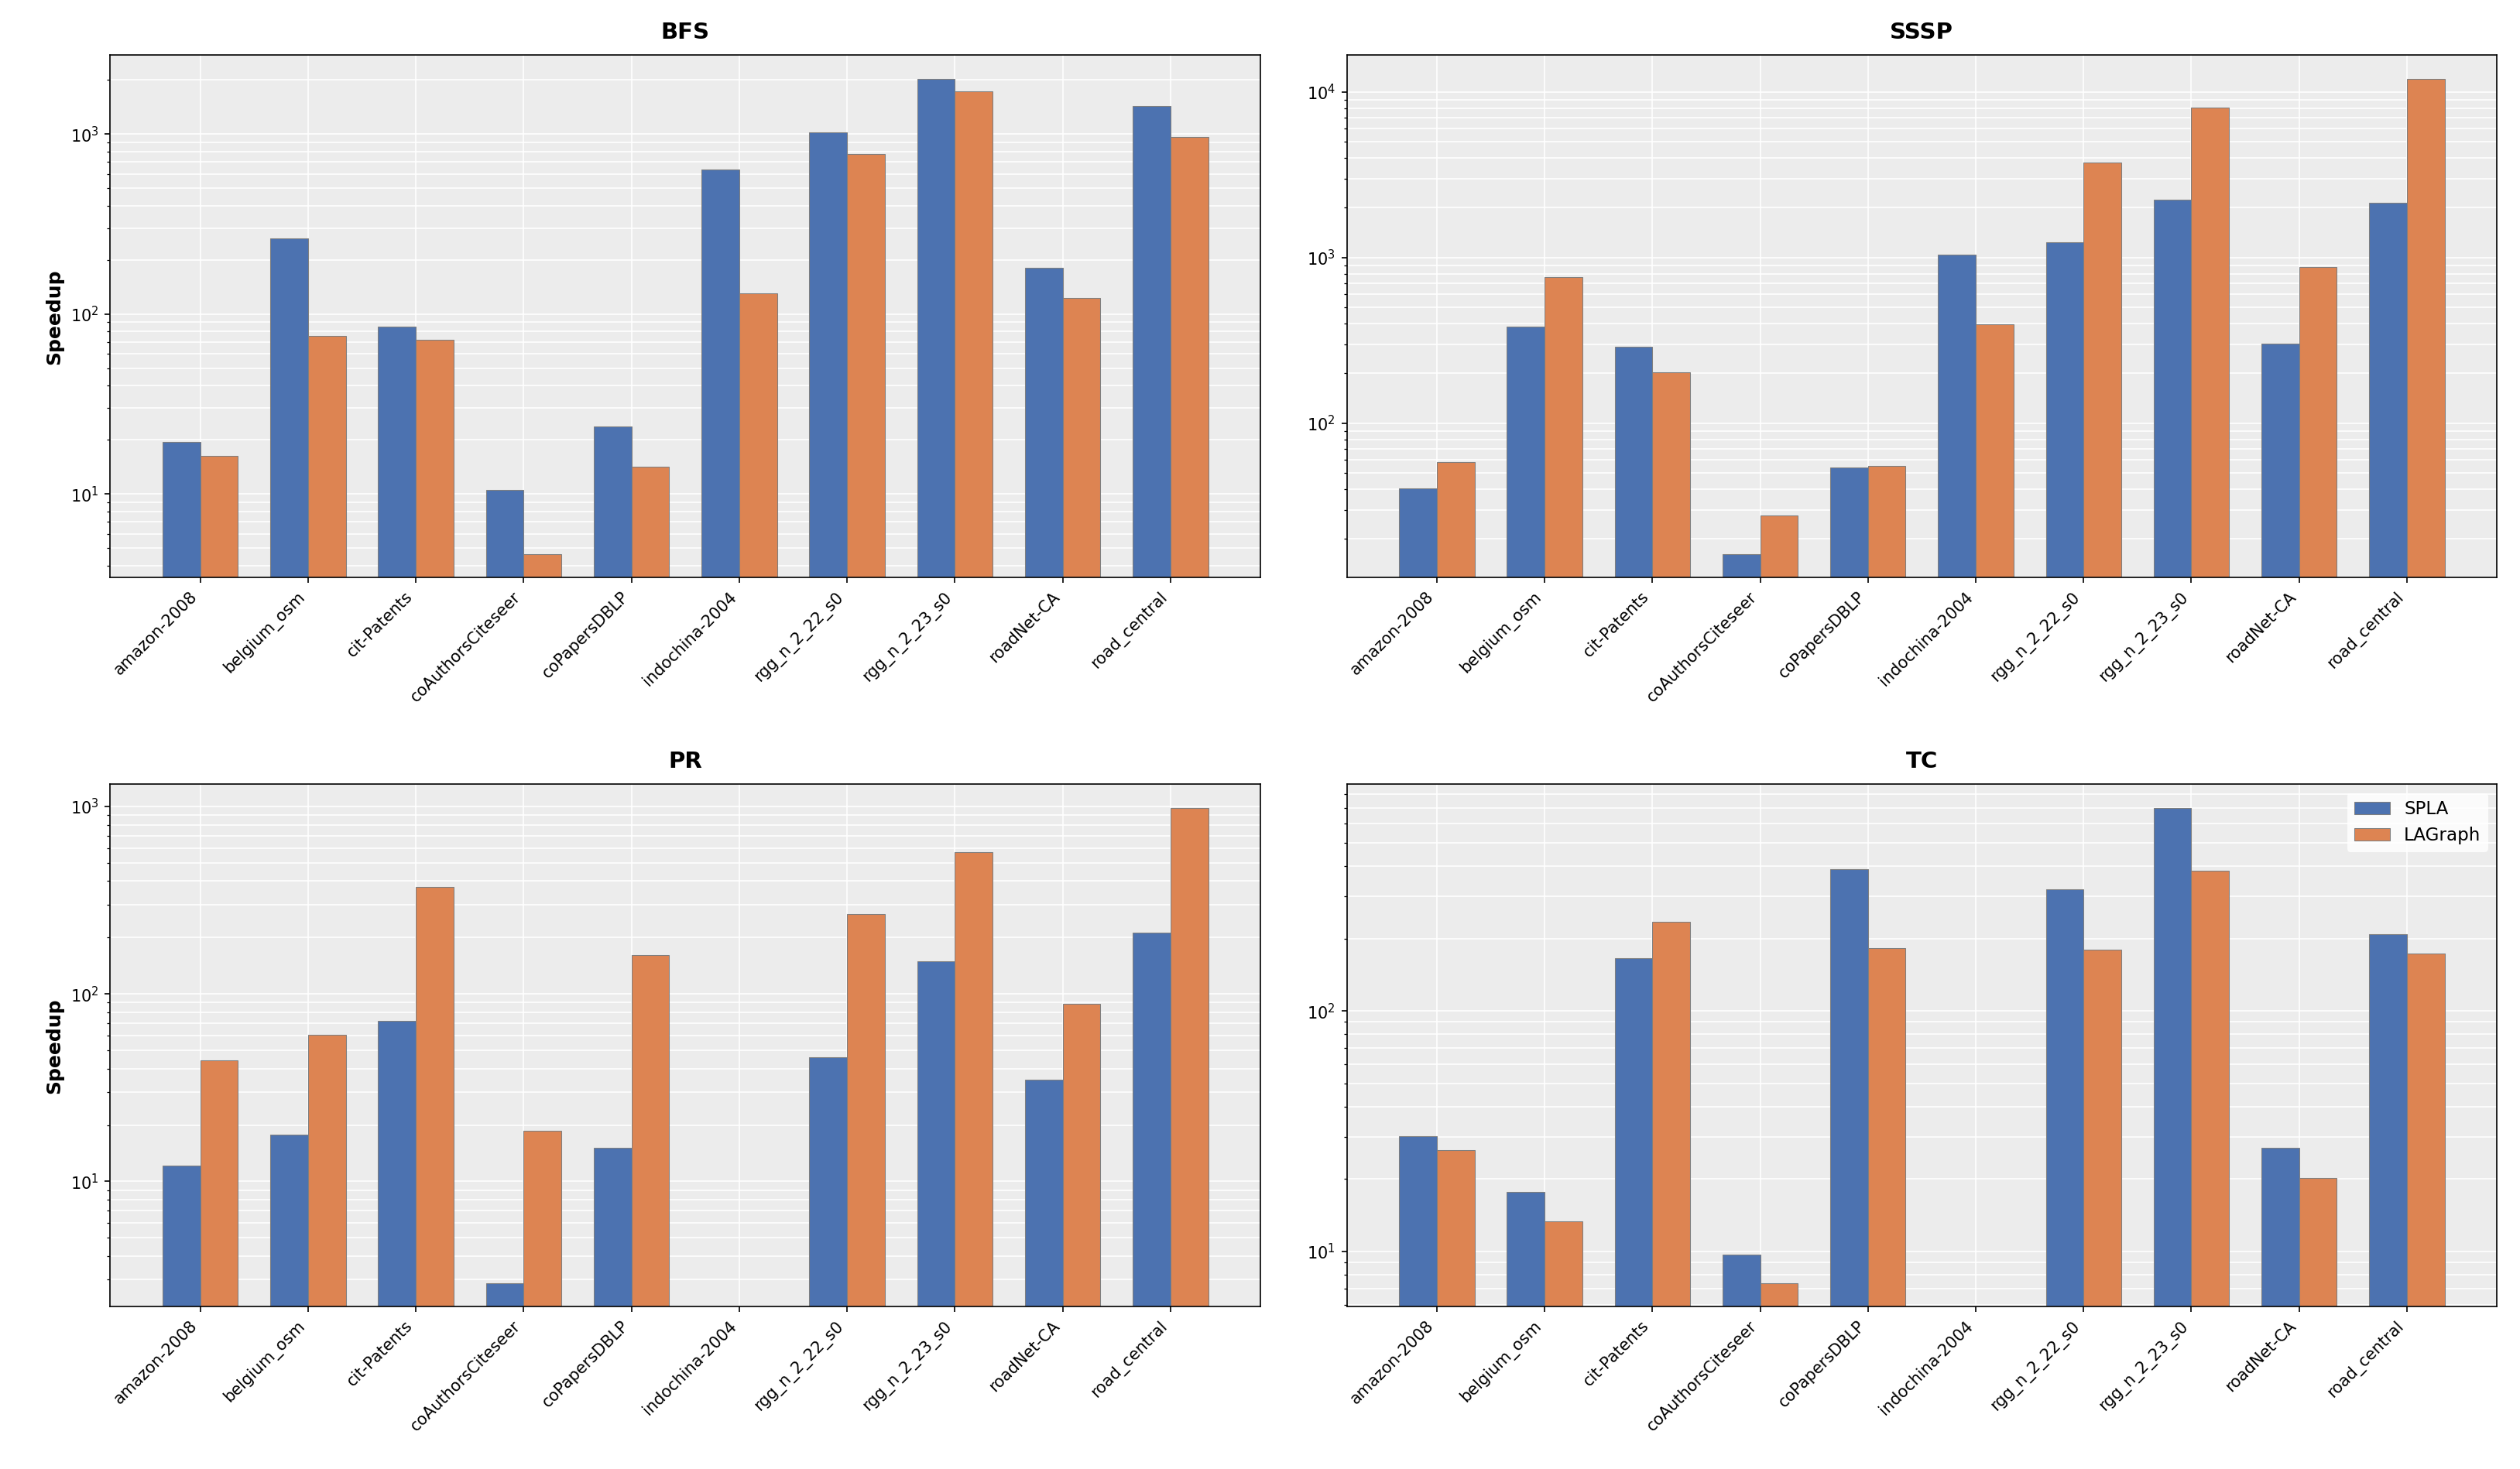
\includegraphics[width=0.8\textwidth]{graphic.png}
		\caption{Сравнение времени выполнения алгоритмов}
		\label{fig:pr_plot}
	\end{figure}
	
	По графику следует сравнить время выполнения алгоритмов на Spla и Lagraph и определить соответствие визуализированных результатов приведённым выше результатам эксперимента.
	
	Все результаты замеров и их средние значения доступны по ссылке: \url{https://drive.google.com/drive/u/1/folders/1J8WVkNs5ktG_Cv5sLw4bG_vfufb1ZyvR}
	
	\section{Заключение}
	
	В ходе выполнения работы получены следующие результаты:
	
	\begin{itemize}
		\item Проведено сравнительное тестирование библиотек Spla (GPU/OpenCL) и Lagraph (CPU) на 10 различных графах из репозитория \texttt{graph-bench}.
		\item Выявлено, что для алгоритмов с высокой степенью параллелизма и регулярными паттернами доступа к памяти (PageRank, SSSP на дорожных сетях) использование Spla обеспечивает ускорение до 10 раз по сравнению с CPU-аналогом.
		\item Показано, что для алгоритмов с нерегулярным обходом графа (BFS, Triangle Counting) более предпочтительным является использование Lagraph на CPU.
	\end{itemize}
	
	\begin{thebibliography}{99}
		\bibitem{spla_orig} Исходный код библиотеки Spla [Электронный ресурс]. URL: https://github.com/SparseLinearAlgebra/spla (дата обращения: 20.09.2026).
		\bibitem{graphbench} Исходный код библиотеки graph-bench [Электронный ресурс]. URL: https://github.com/EgorOrachyov/graph-bench (дата обращения: 20.09.2026).
		\bibitem{lagraph} Исходный код библиотеки LAGraph [Электронный ресурс]. URL: https://github.com/GraphBLAS/LAGraph (дата обращения: 20.09.2026).
		\bibitem{graphblas} GraphBLAS [Электронный ресурс]. URL: https://graphblas.org/ (дата обращения: 20.09.2026).
		\bibitem{suitesparse} SuiteSparse Matrix Collection [Электронный ресурс]. URL: https://sparse.tamu.edu/ (дата обращения: 20.09.2026).
	\end{thebibliography}
	
	Ссылка на репозиторий URL: \url{https://github.com/Lintari/Spla_experiments/tree/main}
	
\end{document}
```
